%++++++++++++++++++++++++++++++++++++++++
\documentclass[article, 12pt]{article}
\usepackage{float}
\usepackage{setspace}
\usepackage{tabu} % extra features for tabular environment
\usepackage{amsmath}  % improve math presentation
\usepackage{graphicx} % takes care of graphic including machinery
\usepackage[margin=1in]{geometry} % decreases margins
\usepackage{cite} % takes care of citations
\usepackage[final]{hyperref} % adds hyper links inside the generated pdf file
\usepackage{tikz}
\usepackage{caption} 
\usepackage{fancyhdr}
\usepackage{amssymb} % symbols like /therefore
\usepackage{amsthm} % proofs
\usepackage{enumerate} % lettered lists
\usepackage{mathtools} % macros
\usepackage[ all]{xy} % for diagrams
\usepackage{tkz-graph}
\usetikzlibrary{knots}
\usetikzlibrary{scopes}
% \usepackage{xcolor} \pagecolor[rgb]{0.12549019607,0.1294117647,0.13725490196} \color[rgb]{0.82352941176,0.76862745098,0.62745098039} % dark theme
\theoremstyle{definition}
\newtheorem{example}{Example}[subsubsection]
\newtheorem*{remark}{Remark}
\newtheorem{theorem}{Theorem}[subsubsection]
\newtheorem{definition}{Definition}[subsubsection]
\newtheorem{corollary}{Corollary}[subsubsection]
\hypersetup{
	colorlinks=false,      % false: boxed links; true: colored links
	linkcolor=blue,        % color of internal links
	citecolor=blue,        % color of links to bibliography
	filecolor=magenta,     % color of file links
	urlcolor=blue         
}
\usepackage{physics}
\usepackage{siunitx}
\usepackage{tikz,pgfplots}
\usepackage[outline]{contour} % glow around text
\usetikzlibrary{calc}
\usetikzlibrary{angles,quotes} % for pic
\usetikzlibrary{arrows.meta}
\tikzset{>=latex} % for LaTeX arrow head
\contourlength{1.2pt}

\colorlet{xcol}{blue!70!black}
\colorlet{vcol}{green!60!black}
\colorlet{myred}{red!70!black}
\colorlet{myblue}{blue!70!black}
\colorlet{mygreen}{green!70!black}
\colorlet{mydarkred}{myred!70!black}
\colorlet{mydarkblue}{myblue!60!black}
\colorlet{mydarkgreen}{mygreen!60!black}
\colorlet{acol}{red!50!blue!80!black!80}
\tikzstyle{CM}=[red!40!black,fill=red!80!black!80]
\tikzstyle{xline}=[xcol,thick,smooth]
\tikzstyle{mass}=[line width=0.6,red!30!black,fill=red!40!black!10,rounded corners=1,
                  top color=red!40!black!20,bottom color=red!40!black!10,shading angle=20]
\tikzstyle{faded mass}=[dashed,line width=0.1,red!30!black!40,fill=red!40!black!10,rounded corners=1,
                        top color=red!40!black!10,bottom color=red!40!black!10,shading angle=20]
\tikzstyle{rope}=[brown!70!black,very thick,line cap=round]
\def\rope#1{ \draw[black,line width=1.4] #1; \draw[rope,line width=1.1] #1; }
\tikzstyle{force}=[->,myred,very thick,line cap=round]
\tikzstyle{velocity}=[->,vcol,very thick,line cap=round]
\tikzstyle{Fproj}=[force,myred!40]
\tikzstyle{myarr}=[-{Latex[length=3,width=2]},thin]
\def\tick#1#2{\draw[thick] (#1)++(#2:0.12) --++ (#2-180:0.24)}
\DeclareMathOperator{\sn}{sn}
\DeclareMathOperator{\cn}{cn}
\DeclareMathOperator{\dn}{dn}
\def\N{80} % number of samples in plots


\usepackage{titling}
\renewcommand\maketitlehooka{\null\mbox{}\vfill}
\renewcommand\maketitlehookd{\vfill\null}
\usepackage{siunitx} % units
\usepackage{verbatim} 
\newcommand{\courseNumber}{MATH 1700}
\newcommand{\courseName}{Ideas in Mathematics}
\newcommand{\professor}{Professor Rimmer}
\newcommand{\psetName}{Worksheet 6: Knot Theory Second Submission}
\newcommand{\dueDate}{Due: March 22, 2023}
\newcommand{\name}{Denny Cao}
\pagestyle{fancy}
\fancyhf{}% clears all header and footer fields
\fancyfoot[C]{--~\thepage~--}
\renewcommand*{\headrulewidth}{0.4pt}
\renewcommand*{\footrulewidth}{0pt}
\lhead{\name}
\chead{\courseNumber: \courseName}
\rhead{\professor}

% new theorem for questions and answers

\newtheorem{question}{Question}

\newtheorem{answer}{Answer}

\fancypagestyle{plain}{%
  \fancyhf{}% clears all header and footer fields
  \fancyfoot[C]{--~\thepage~--}%
  \renewcommand*{\headrulewidth}{0pt}%
  \renewcommand*{\footrulewidth}{0pt}%
}

% Shortcuts
\DeclarePairedDelimiter\ceil{\lceil}{\rceil} % ceil function
\DeclarePairedDelimiter\floor{\lfloor}{\rfloor} % floor function

\DeclarePairedDelimiter\paren{(}{)} % parenthesis

\newcommand{\df}{\displaystyle\frac} % displaystyle fraction
\newcommand{\qeq}{\overset{?}{=}} % questionable equality

\newcommand{\Mod}[1]{\;\mathrm{mod}\; #1} % modulo operator

\newcommand{\comp}{\circ} % composition

% Sets
\DeclarePairedDelimiter\set{\{}{\}}
\newcommand{\unite}{\cup}
\newcommand{\inter}{\cap}

\newcommand{\reals}{\mathbb{R}} % real numbers: textbook is Z^+ and 0
\newcommand{\ints}{\mathbb{Z}}
\newcommand{\nats}{\mathbb{N}}
\newcommand{\rats}{\mathbb{Q}}

\newcommand{\degree}{^\circ}

% Counting
\newcommand\perm[2][^n]{\prescript{#1\mkern-2.5mu}{}P_{#2}}
\newcommand\comb[2][^n]{\prescript{#1\mkern-0.5mu}{}C_{#2}}

% Relations
\newcommand{\rel}{\mathcal{R}} % relation

\setlength\parindent{0pt}

% Directed Graphs
\usetikzlibrary{arrows}
\tikzset{vertex/.style = {shape=circle,draw, minimum size=1.5em,
inner sep=0pt, outer sep=0pt}}
\tikzset{edge/.style = {->,> = latex'}}

% Contradiction
\newcommand{\contradiction}{{\hbox{%
    \setbox0=\hbox{$\mkern-3mu\times\mkern-3mu$}%
    \setbox1=\hbox to0pt{\hss$\times$\hss}%
    \copy0\raisebox{0.5\wd0}{\copy1}\raisebox{-0.5\wd0}{\box1}\box0
}}}

% Sign Charts
\newdimen\tcolw \tcolw=2.5em % the column width
\edef\ecatcode{\catcode`&=\the\catcode`&\relax}\catcode`&=4
\def\sgchart#1#2{\vbox{\offinterlineskip\halign{\hfil##\quad&##\hfil\crcr\sgchartA#2,:,%
   \omit\sgchartR&\kern.2pt\sgchartS{.5\tcolw}\relax\sgchartE#1,\relax,%
   \sgchartS{.5\tcolw}\relax\cr
   \noalign{\kern2pt}&\def~{}\kern.5\tcolw\sgchartD#1,\relax,\cr}}}
\def\sgchartA#1:#2,{\cr\ifx,#1,\else $#1$&\sgchartB#2{}\expandafter\sgchartA\fi}
\def\sgchartB#1{\hbox to\tcolw{\hss$#1$\hss}\sgchartC}
\def\sgchartC#1{\ifx,#1,\else
   \strut\vrule\kern-.4pt\hbox to\tcolw{\hss$#1$\hss}\expandafter\sgchartC\fi}
\def\sgchartD#1#2,{\ifx\relax#1\else\hbox to\tcolw{\hss$#1#2$\hss}\expandafter\sgchartD\fi}
\def\sgchartE#1#2,{\ifx\relax#1\else
    \ifx~#1\sgchartS\tcolw\circ \else\sgchartS\tcolw\bullet\fi \expandafter\sgchartE\fi}
\def\sgchartR{\leaders\vrule height2.8pt depth-2.4pt\hfil}
\def\sgchartS#1#2{\hbox to#1{\kern-.2pt\sgchartR \ifx\relax#2\else
   \kern-.7pt$#2$\kern-.7pt\sgchartR\fi\kern-.2pt}}
\ecatcode
%++++++++++++++++++++++++++++++++++++++++
% title stuff

\makeatletter
\renewcommand{\maketitle}{\bgroup\setlength{\parindent}{0pt}
    \begin{flushleft}
        \textbf{\@title} \\ \vskip0.2cm
        \begingroup
            \fontsize{14pt}{12pt}\selectfont
            \courseNumber: \courseName 
            \vskip0.3cm 
            \professor
        \endgroup \vskip0.3cm
        \dueDate \hfill\rlap{}\bf{\name} \\ \vskip0.1cm
        \hrulefill
    \end{flushleft}\egroup 
}
\makeatother

\title{\Large\bf{\psetName}}

\begin{document}
    \maketitle
    \thispagestyle{plain}
    % Question 1
    \begin{question}
        Is it possible to switch some crossings in the Borromean rings to obtain a trefoil knot? Why or why not? If so, how many switches are needed? (Note that by switching a crossing, we mean changing which strand goes over/in front and which goes under/behind.)        
    \end{question}
    % Answer 1
    \begin{answer}  
        No, it is not possible to switch some crossings in the Borromean rings to obtain a trefoil knot. 
        
        \begin{proof}
            We label the crossings and strands in the Borromean rings as follows:
            \begin{figure}[H]
                \centering
                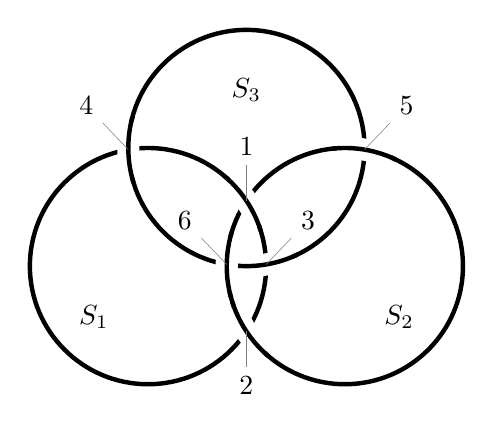
\begin{tikzpicture}
                    \begin{knot}[
                        draft mode=crossings,
                        clip width=5,
                        flip crossing=2,
                        flip crossing=3,
                        flip crossing=4,
                        draft/crossing label/.style={
                            text=black,
                            pin position=90,
                        },
                        draft/crossing 6 label/.style={
                            text=black,
                            pin position=135,
                        },
                        draft/crossing 3 label/.style={
                            text=black,
                            pin position=45,
                        },
                        draft/crossing 2 label/.style={
                            text=black,
                            pin position=-90,
                        },
                        draft/crossing 4 label/.style={
                            text=black,
                            pin position=135,
                        },
                        draft/crossing 5 label/.style={
                            text=black,
                            pin position=45,
                        },
                        draft/strand label/.style={
                            fill opacity=0,
                        },
                    ]                    
                        \strand[black, ultra thick] (0,2) circle (1.5) node[label={[label distance=0.3cm]225:$S_1$}] {};
                        \strand[black, ultra thick] (2.5,2) circle (1.5) node[label={[label distance=0.3cm]315:$S_2$}] {};
                        \strand[black, ultra thick] (1.25,3.5) circle (1.5) node[label={[label distance=0.3cm]90:$S_3$}] {};
                    \end{knot}
                \end{tikzpicture}
            \end{figure}
            A property of Borromean rings is that the three interlocked strands cannot be separated. As a trefoil is a single strand, without any crossing switches, it is not possible to obtain a trefoil from the Borromean rings. 
            \\[12pt]
            If we were to switch crossings to result in a single strand, we would need to switch crossings 2, 3, and 4. However, this would result in the following diagram:
            \begin{figure}[H]
                \centering
                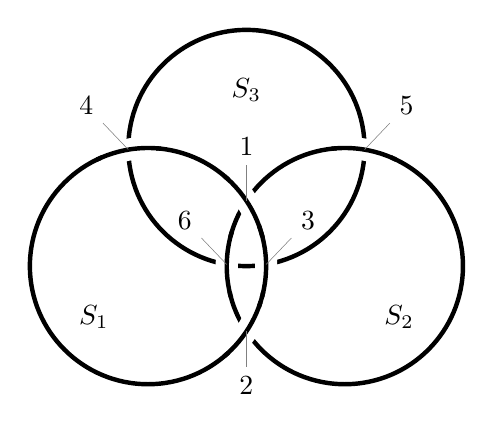
\begin{tikzpicture}
                    \begin{knot}[
                        draft mode=crossings,
                        clip width=5,
                        draft/crossing label/.style={
                            text=black,
                            pin position=90,
                        },
                        draft/crossing 6 label/.style={
                            text=black,
                            pin position=135,
                        },
                        draft/crossing 3 label/.style={
                            text=black,
                            pin position=45,
                        },
                        draft/crossing 2 label/.style={
                            text=black,
                            pin position=-90,
                        },
                        draft/crossing 4 label/.style={
                            text=black,
                            pin position=135,
                        },
                        draft/crossing 5 label/.style={
                            text=black,
                            pin position=45,
                        },
                        draft/strand label/.style={
                            fill opacity=0,
                        },
                    ]                    
                        \strand[black, ultra thick] (0,2) circle (1.5) node[label={[label distance=0.3cm]225:$S_1$}] {};
                        \strand[black, ultra thick] (2.5,2) circle (1.5) node[label={[label distance=0.3cm]315:$S_2$}] {};
                        \strand[black, ultra thick] (1.25,3.5) circle (1.5) node[label={[label distance=0.3cm]90:$S_3$}] {};
                    \end{knot}
                \end{tikzpicture}
            \end{figure}
            With a Reidemeister move, the three strands can be separated, resulting in 3 unknots:
            \begin{figure}[H]
                \centering
                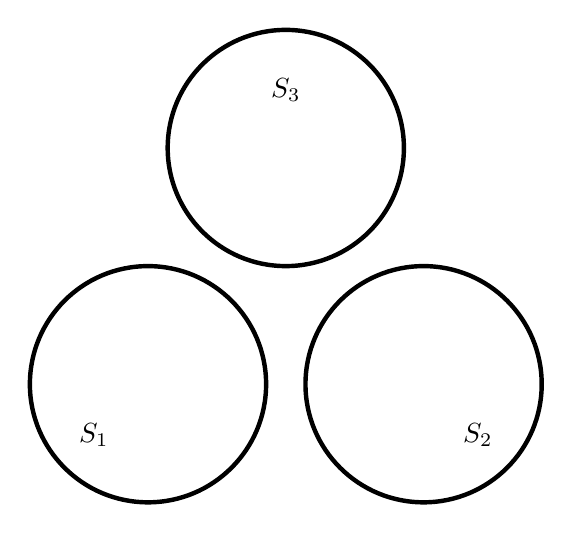
\begin{tikzpicture}
                    \begin{knot}[
                        clip width=5,
                    ]                    
                        \strand[black, ultra thick] (0,2) circle (1.5) node[label={[label distance=0.3cm]225:$S_1$}] {};
                        \strand[black, ultra thick] (3.5,2) circle (1.5) node[label={[label distance=0.3cm]315:$S_2$}] {};
                        \strand[black, ultra thick] (1.75,5) circle (1.5) node[label={[label distance=0.3cm]90:$S_3$}] {};
                    \end{knot}
                \end{tikzpicture}
            \end{figure}
            As a trefoil has the invariant of being three-colored and unknots are not, a trefoil cannot be obtained from the Borromean rings by switching crossings.
        \end{proof}
    \end{answer}

    % Question 2
    \begin{question}
        Is it possible to switch some number of crossings in the trefoil knot to obtain an unknot? If so, what is the minimum number of switches needed?
    \end{question}
    % Answer 2
    \begin{answer}
        Yes, it is possible to switch some crossings in the trefoil knot to obtain an unknot. The minimum number of switches needed is 2.
        \begin{proof}
            We label the crossings in the trefoil as follows:
            \begin{figure}[H]
                \centering
                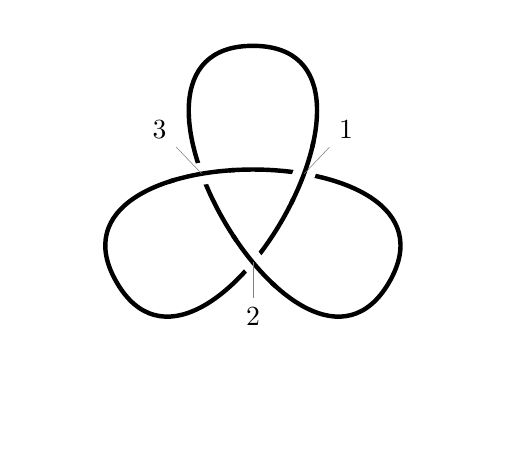
\begin{tikzpicture}
                    \begin{knot}[
                        draft mode=crossings,
                        clip width=5,
                        consider self intersections=true,
                      %  draft mode=crossings,
                        flip crossing=2,
                        only when rendering/.style={
                      %    show curve controls
                        },
                        draft/crossing label/.style={
                            text=black,
                            pin position=90,
                        },
                        draft/crossing 1 label/.style={
                            text=black,
                            pin position=45,
                        },
                        draft/crossing 2 label/.style={
                            text=black,
                            pin position=-90,
                        },
                        draft/crossing 3 label/.style={
                            text=black,
                            pin position=135,
                        },
                        draft/strand label/.style={
                            fill opacity=0,
                        },
                        ]
                      \strand[black, ultra thick] (0,2) .. controls +(2.2,0) and +(120:-2.2) .. (210:2) .. controls +(120:2.2) and +(60:2.2) .. (-30:2) .. controls +(60:-2.2) and +(-2.2,0) .. (0,2);
                      \end{knot}
                \end{tikzpicture}
            \end{figure}
            We can switch crossings 2 and 3 to obtain the following diagram:
            \begin{figure}[H]
                \centering
                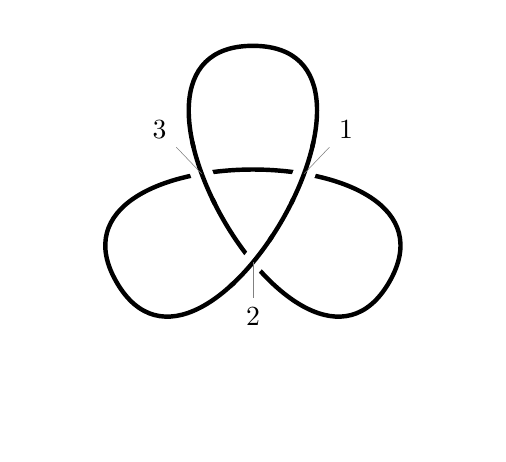
\begin{tikzpicture}
                    \begin{knot}[
                        draft mode=crossings,
                        clip width=5,
                        consider self intersections=true,
                      %  draft mode=crossings,
                        flip crossing=3,
                        only when rendering/.style={
                      %    show curve controls
                        },
                        draft/crossing label/.style={
                            text=black,
                            pin position=90,
                        },
                        draft/crossing 1 label/.style={
                            text=black,
                            pin position=45,
                        },
                        draft/crossing 2 label/.style={
                            text=black,
                            pin position=-90,
                        },
                        draft/crossing 3 label/.style={
                            text=black,
                            pin position=135,
                        },
                        draft/strand label/.style={
                            fill opacity=0,
                        },
                        ]
                      \strand[black, ultra thick] (0,2) .. controls +(2.2,0) and +(120:-2.2) .. (210:2) .. controls +(120:2.2) and +(60:2.2) .. (-30:2) .. controls +(60:-2.2) and +(-2.2,0) .. (0,2);
                      \end{knot}
                \end{tikzpicture}
            \end{figure}
            With Reidemeister moves, we can form the unknot. Thus, it is possible to switch 2 crossings of the trefoil knot to obtain an unknot. It is impossible to switch 1 crossing of the trefoil knot to obtain an unknot, as it has the invariant of being three-colored, while the unknot does not. Thus, the minimum number of switches needed is 2.
        \end{proof}
    \end{answer}

    % Question 3
    \begin{question}
        For each of the knot diagrams on page 365 of your book (reproduced on the next page), give a sequence of Reidemeister to obtain another diagram of the same knot which you feel is as simple as possible. In each case, how do you know you can't do any better?
    \end{question}

    % Answer 3
    \begin{answer} \ 

        \begin{itemize}
            \item \ \\ 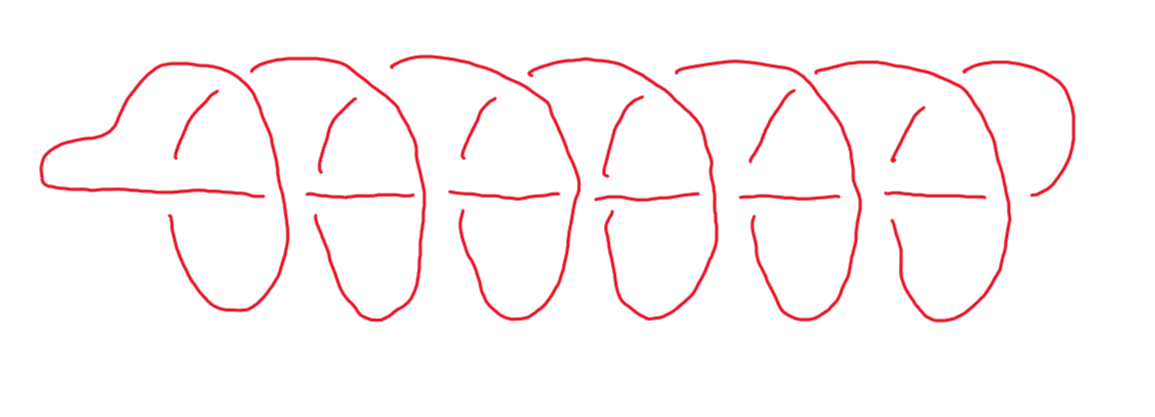
\includegraphics[scale=.4]{slinky.png}
            
            It is possible to obtain the unknot from the slinky knot by ``unwrapping'' the knot through slide moves. 
            \item \ \\ 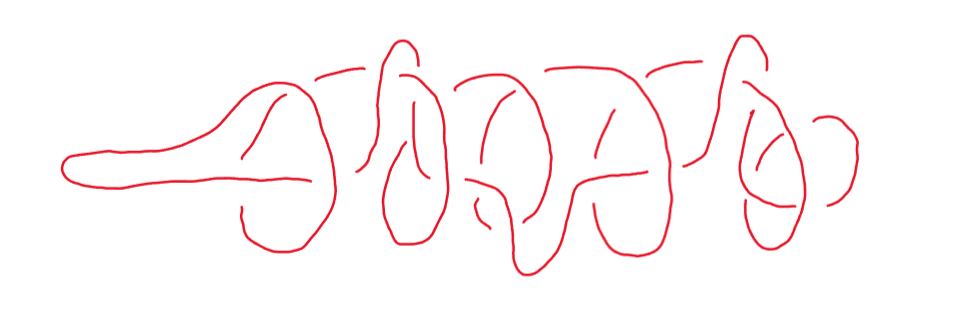
\includegraphics[scale=.4]{croc.png}
            
            We do the following Reidemeister moves to obtain the unknot:

            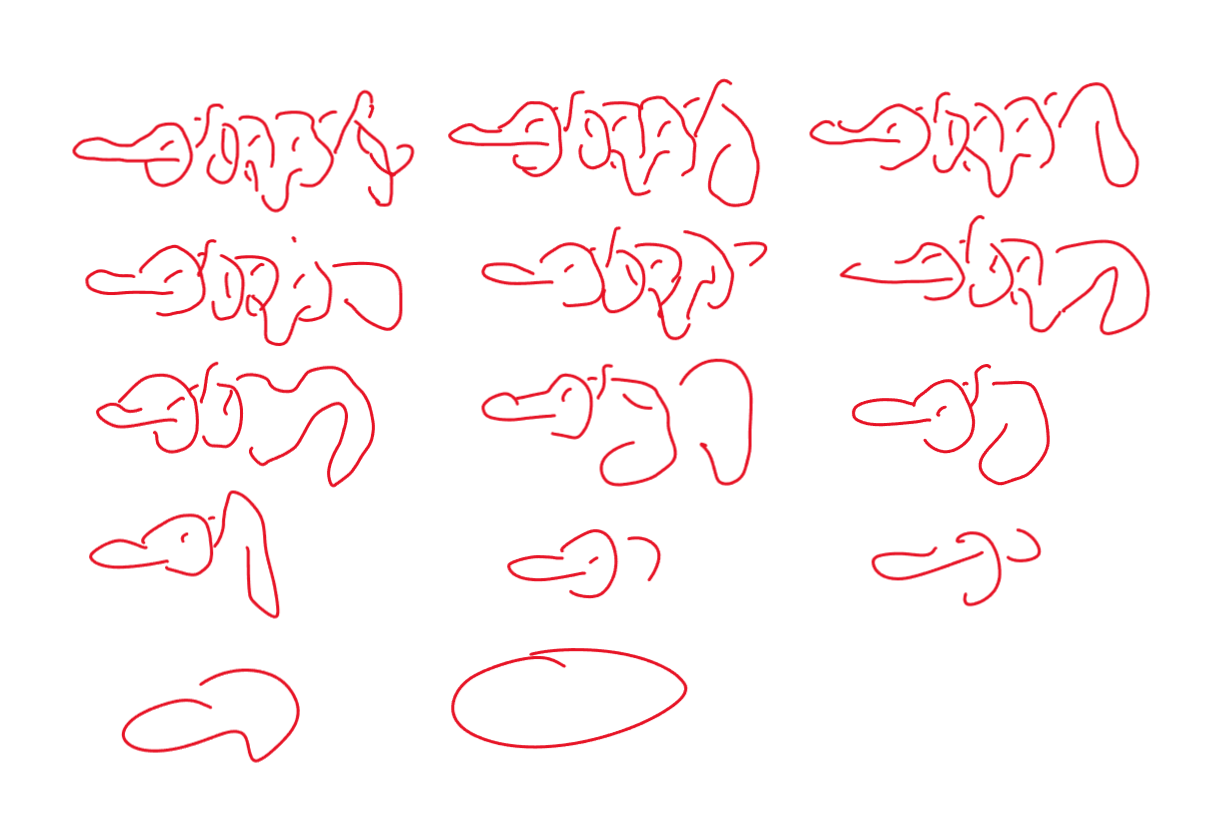
\includegraphics[scale=.3]{wtf.png}
            \item \ \\ 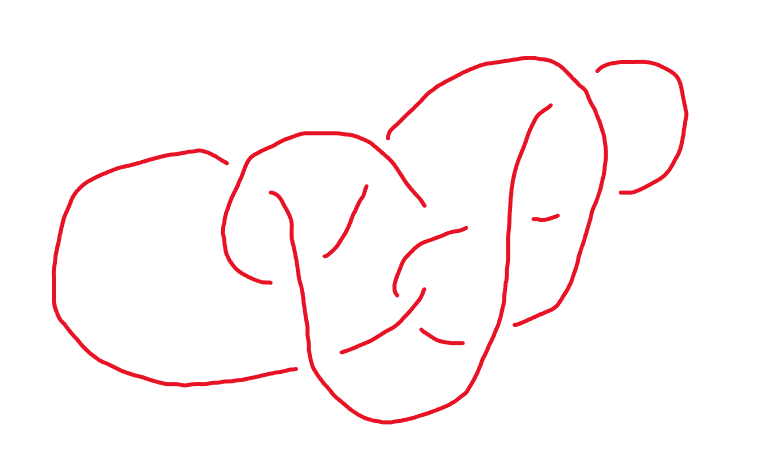
\includegraphics[scale=.4]{elephant.png}
            
            We do the following Reidemeister moves to obtain the unknot:

            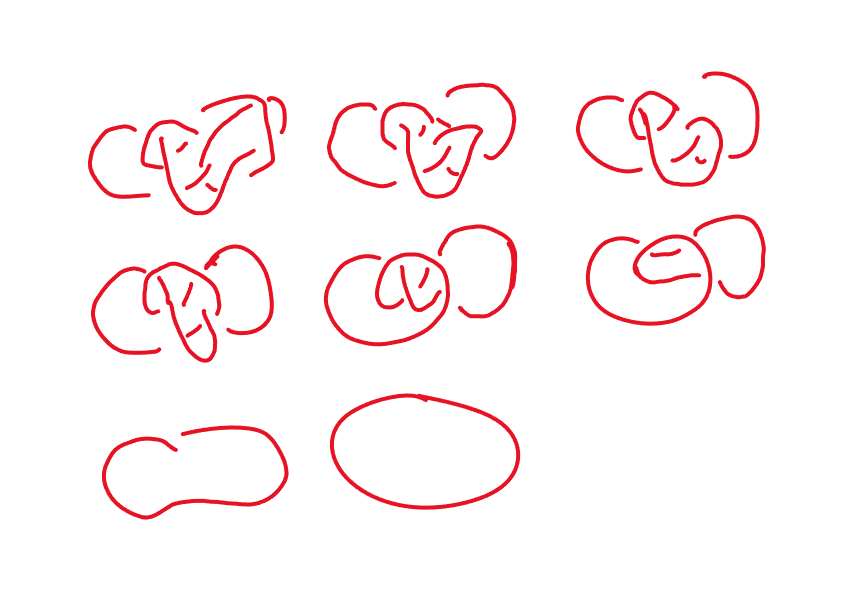
\includegraphics[scale=.4]{wtf2.png}
            \item \ \\ 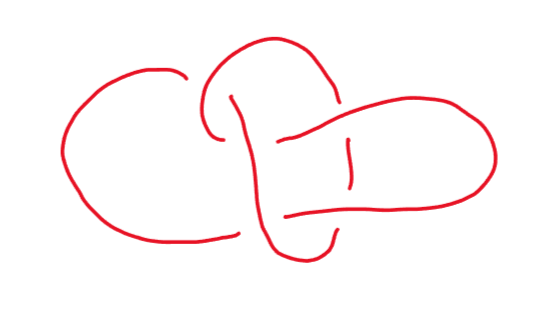
\includegraphics[scale=.4]{pacifier.png}
            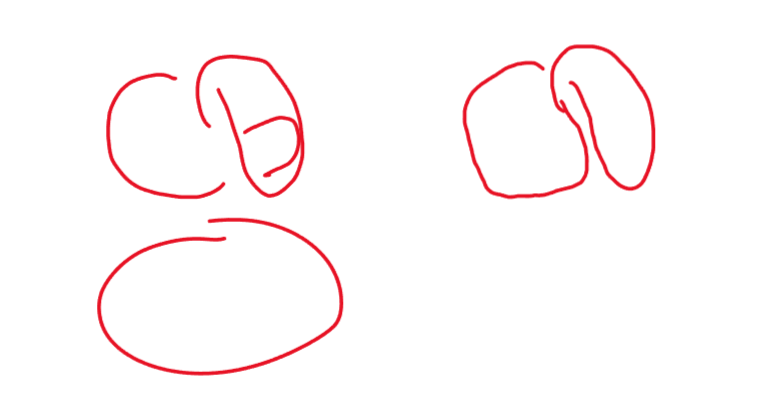
\includegraphics[scale=.4]{wtf3.png}
        \end{itemize}
        As we can see, the Reidemeister moves we performed to obtain the unknot from each of the diagrams are as simple as possible. We can't do any better because it is prime.
    \end{answer}

    % Question 4    
    \begin{question}
        Are the figure-eight, cinquefoil knot, and three-twist knot (entries 41, 51, and 52 on your table, respectively) three-colorable?
    \end{question}
    % Answer 4
    \begin{answer}
        No, they are not three-colorable. The coloring for the three figures are as follows:
        \begin{itemize}
            \item \ \\ 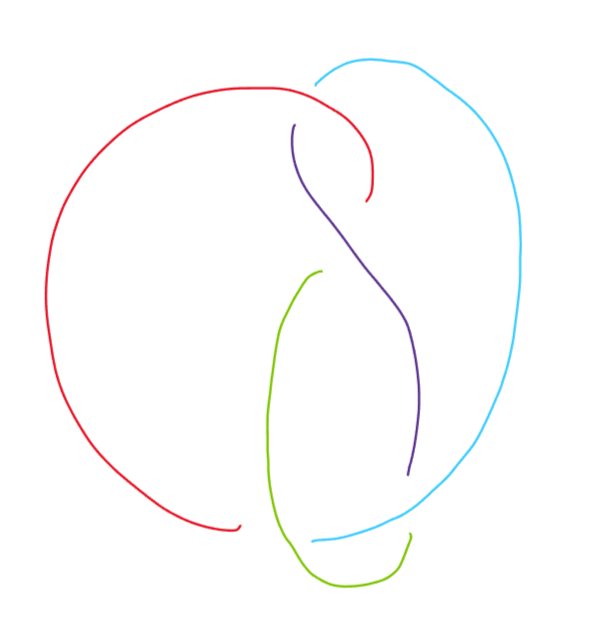
\includegraphics[scale=.2]{figure_8.png}
            \item \ \\ 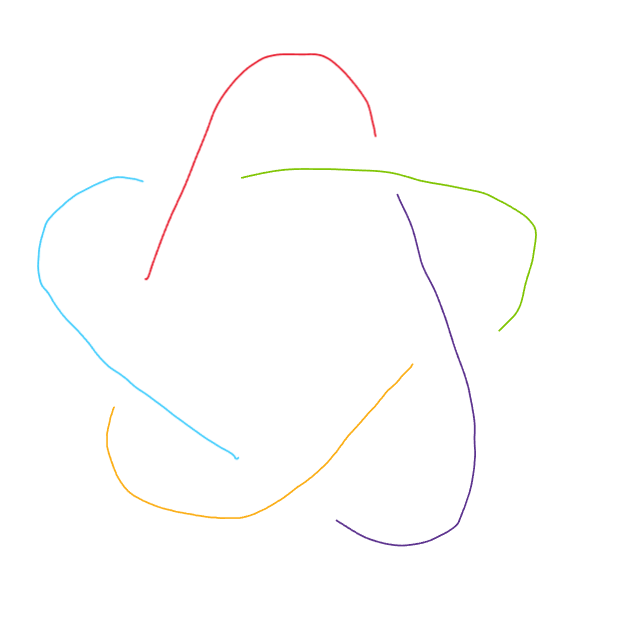
\includegraphics[scale=.2]{star.png}
            \item \ \\ 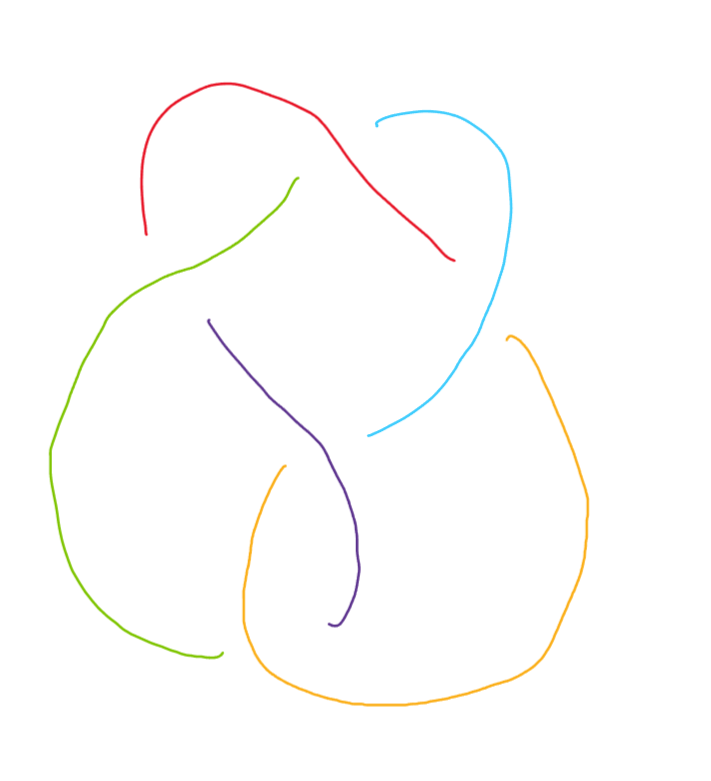
\includegraphics[scale=.2]{pret.png}
        \end{itemize}
    \end{answer}

    % Question 5
    \begin{question}
        Show that for any number $n > 2$, there is a knot diagram of the trefoil with exactly $n$ crossings.    
    \end{question}
    % Answer 5
    \begin{answer}
        \begin{proof}
            To construct a trefoil knot with exactly $n$ crossings, we can start with the standard trefoil diagram with three crossings and then add $n-3$ additional crossings to it by twisting one of the strands around itself $n-3$ times. The total number of crossings is $n$.
        \end{proof}
    \end{answer}

    % Question 6
    \begin{question}
        A knot diagram is called \textit{alternating} if you can start anywhere in the knot, and alternate undercrossing and overcrossings until you are back where you started. Show that the usual picture of the trefoil (as shown in the top left corner of the table of knots on Canvas) is alternating. How is this possible for a knot diagram with an odd number of crossings to be alternating?
    \end{question}
    % Answer 6
    \begin{answer}
        \begin{proof}
            We label the crossings in the trefoil as follows:
            \begin{figure}[H]
                \centering
                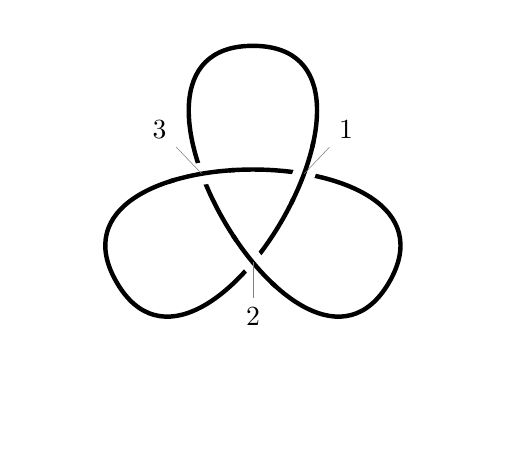
\begin{tikzpicture}
                    \begin{knot}[
                        draft mode=crossings,
                        clip width=5,
                        consider self intersections=true,
                      %  draft mode=crossings,
                        flip crossing=2,
                        only when rendering/.style={
                      %    show curve controls
                        },
                        draft/crossing label/.style={
                            text=black,
                            pin position=90,
                        },
                        draft/crossing 1 label/.style={
                            text=black,
                            pin position=45,
                        },
                        draft/crossing 2 label/.style={
                            text=black,
                            pin position=-90,
                        },
                        draft/crossing 3 label/.style={
                            text=black,
                            pin position=135,
                        },
                        draft/strand label/.style={
                            fill opacity=0,
                        },
                        ]
                      \strand[black, ultra thick] (0,2) .. controls +(2.2,0) and +(120:-2.2) .. (210:2) .. controls +(120:2.2) and +(60:2.2) .. (-30:2) .. controls +(60:-2.2) and +(-2.2,0) .. (0,2);
                      \end{knot}
                \end{tikzpicture}
            \end{figure}
        We can see that the crossings alternate between over and under as we travel along the knot, as 1 is over, 2 is under, and 3 is over. Thus, the trefoil is alternating.
        \\[12pt]
        It is possible for a knot diagram with an odd number of crossings to be alternating because, by linking back to the starting point, alternating crossings are possible.
    \end{proof}
    \end{answer}    
    
    % Question 7
    \begin{question}
        Consider the link below. 

        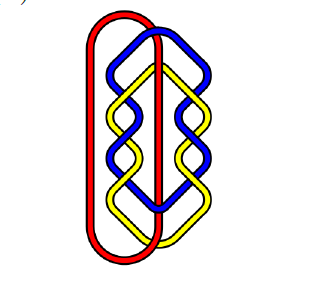
\includegraphics[scale=.4]{fullpaper.png}
        
        It is \textit{not} equivalent to the Borromean rings. Show that after removing any one of the strands, it is possible to separate the other two using Reidemeister moves.
    \end{question}

    % Answer 7
    \begin{answer}
        \begin{proof}
            The following are how the link would look like after removing one of the strands:
            
            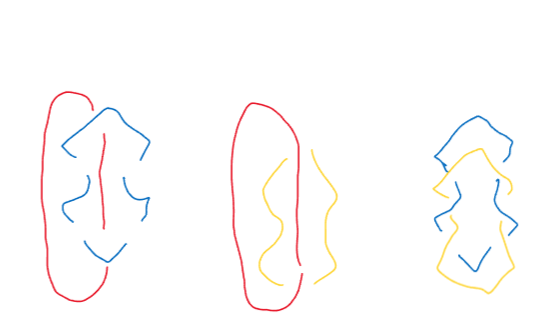
\includegraphics[scale=.4]{paperclip_and_shit.png}

            We can see that after removing one of the strands, it is possible to separate the other two using Reidemeister moves. In the first, we can separate the two strands by performing a slide move on the strand on the left. In the second, we can separate the two strands by performing a slide move on the strand on the left as well. In the third, we can separate the two strands by performing a poke and then a twist on the blue strand. 
        \end{proof}
    \end{answer}
    \section*{Reflection}
    \textbf{Identify at least one wrong or failed idea that turned out to be helpful or enlightening in some way. For instance, that idea might have helped you solve a problem, or it may have been the start of a conversation that improved your understanding more generally. You can list one of your own ideas, or an idea that originated with a classmate. (Please give your classmate credit!)}

    Knot theory has been the first topic we've covered that I have not been familiar with, and I received a lot of help working with Larry Huang. For Question 4, I didn't understand how three-colorable knots are defined, as part of the definition is if each intersection has 1 color or three colors. Larry explained how I missed another part of the definition---at least two colors must be used. With this, I now understand why the unknot is not three-corable.
\end{document} 
